\subsection{Primitive and leaf}\label{sec:levers}

Figure~\ref{fig:levers} and Table~\ref{tab:levers} split, cloud by cloud, the gap between a library default and the fastest structure the search finds into two steps. Three variants are compared on the held-out half of every cloud: the engine's octree default (16 levels, leaf 32); the \emph{best primitive}, the fastest of the engine's nine primitives at their default parameters (leaf 32, default split rule); and the \emph{tuned} structure, the fastest single structure of any leaf, depth and split rule. Every ratio is between variants measured on the same cloud under the same protocol.

\begin{figure}[tb]
\centering
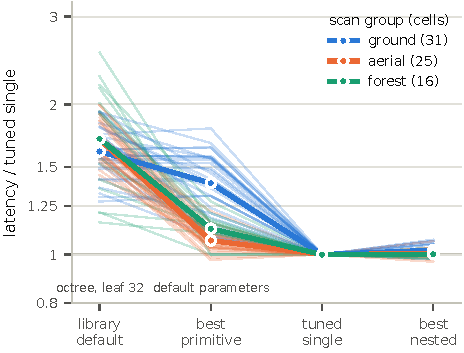
\includegraphics[width=\linewidth]{figures/fig_levers}
\caption{From library default to tuned structure. For each of the \nCells{} held-out clouds, the latency of the octree default and of the best primitive at default parameters, relative to the tuned structure (thin lines); the thick lines are geometric means per scan group.}
\label{fig:levers}
\end{figure}

\begin{table*}[t]
\centering\footnotesize
\caption{The two steps from a default to the tuned structure, on the held-out half: geometric means of per-cloud latency ratios (above 1: the second variant is faster). \emph{Default}: the engine's octree or median-split kd-tree at leaf 32; \emph{best primitive}: the fastest of the nine primitives at default parameters; \emph{tuned}: the fastest single structure of any leaf, depth and split rule. Clouds up to 50M points were measured on the workstation and from 100M on the server, interleaved protocol; no ratio crosses machines.}
\label{tab:levers}
% generated by scripts/paper/tables.py; do not edit
\begin{tabular}{lrrrrrr}
\toprule
Size or group & clouds & \begin{tabular}[b]{@{}c@{}}octree default\\/ best primitive\end{tabular} & \begin{tabular}[b]{@{}c@{}}kd-tree default\\/ best primitive\end{tabular} & \begin{tabular}[b]{@{}c@{}}best primitive\\/ tuned\end{tabular} & \begin{tabular}[b]{@{}c@{}}octree default\\/ tuned\end{tabular} & \begin{tabular}[b]{@{}c@{}}kd-tree default\\/ tuned\end{tabular} \\
\midrule
1M & 17 & 1.477 & 1.167 & 1.174 & 1.770 & 1.380 \\
5M & 16 & 1.344 & 1.336 & 1.256 & 1.745 & 1.699 \\
25M & 16 & 1.256 & 1.244 & 1.293 & 1.610 & 1.612 \\
50M & 6 & 1.207 & 1.114 & 1.241 & 1.465 & 1.387 \\
100M & 9 & 1.303 & 1.268 & 1.193 & 1.568 & 1.527 \\
250M & 3 & 1.630 & 1.441 & 1.055 & 1.718 & 1.542 \\
500M & 3 & 1.547 & 1.399 & 1.036 & 1.612 & 1.499 \\
1B & 3 & 1.455 & 1.365 & 1.089 & 1.560 & 1.527 \\
\midrule
ground & 31 & 1.175 & 1.124 & 1.391 & 1.610 & 1.550 \\
aerial & 25 & 1.533 & 1.571 & 1.067 & 1.703 & 1.730 \\
forest & 16 & 1.504 & 1.103 & 1.127 & 1.707 & 1.255 \\
\midrule
all & 73 & 1.360 & 1.255 & 1.210 & 1.659 & 1.532 \\
\bottomrule
\end{tabular}

\end{table*}

Over all \nCells{} clouds the octree default is \leverOctreeDefaultTuned$\times$ slower than the tuned structure and the median-split kd-tree default \leverKdDefaultTuned$\times$. Choosing the primitive closes a factor of \leverOctreeDefaultPrimitive{} from the octree and \leverKdDefaultPrimitive{} from the kd-tree; tuning the leaf capacity, the depth and the split rule of that primitive closes a further \leverPrimitiveTuned$\times$.

The two steps trade places between scan groups, which is why one default cannot serve all of them. On the aerial surveys the primitive is the lever: a quadtree beats the octree and kd-tree defaults by half again, because a 2.5-dimensional scene gains nothing from splitting height, and once the quadtree is chosen little is left to tune. On the ground scans the primitive step is small, since a kd-tree at leaf 32 is already close to the octree, and the tuning step is large: these scans want the sliding-midpoint split, deep trees and leaves of 64 to 128 points, none of which a default provides. The forest scans sit between. In every group the two steps together give a factor between 1.5 and 1.8.

The decomposition holds at every size. The default gap does not grow with the cloud: it is as large at one million points as at one billion, so what the defaults miss is not scale but the fit of the primitive and the leaf to the scene. The 250M, 500M and 1B clouds reuse the structure selected at 250M on the same scene and lose nothing by it, so a structure chosen on a quarter of the points transfers to the whole cloud.

\paragraph{The headline panel at 100M, timed sequentially.} The ratios above come from the interleaved protocol, which slows memory-bound trees by up to a fifth (Section~\ref{sec:protocol}). Table~\ref{tab:panel} therefore re-times the nine 100M clouds sequentially, on both page sizes: the two defaults, the flatness rule's pick (Section~\ref{sec:rule}) and the searched best. The picture holds. The octree default is \panelOctreeDefaultBase$\times$ the searched best and the kd-tree default \panelKdDefaultBase$\times$; the rule's pick is \panelRuleBase$\times$, within a few percent on every cloud; and the searched best is \panelPickOracleBase$\times$ the fastest structure of the panel. On 2\,MB pages every ratio moves by a point or two in the same direction, because the variants with more and smaller leaves gain more (Section~\ref{sec:ram}).

\begin{table*}[t]
\centering\footnotesize
\caption{The headline panel at 100 million points, sequential protocol, geometric mean (range, clouds) of per-cloud ratios, on 4\,KiB and on 2\,MB pages. \emph{Searched best}: the structure selected by the search on the other half of the trace; \emph{flatness rule}: the pick of the rule of Section~\ref{sec:rule}. The last row is each structure on 2\,MB pages over itself on 4\,KiB pages.}
\label{tab:panel}
% generated by scripts/paper/tables.py; do not edit
\begin{tabular}{lrr}
\toprule
Ratio & base: 4 KiB pages & huge pages \\
\midrule
octree default / pick & 1.723 (1.31--2.20, $n$=9) & 1.755 (1.32--2.24, $n$=9) \\
kd default / pick & 1.464 (1.14--2.36, $n$=9) & 1.511 (1.15--2.52, $n$=9) \\
rule / pick & 1.009 (1.00--1.04, $n$=9) & 1.041 (1.01--1.08, $n$=9) \\
pick / best single & 1.002 (1.00--1.01, $n$=9) & 1.000 (1.00--1.00, $n$=9) \\
nested / best single & 1.021 (1.00--1.05, $n$=9) & 1.032 (0.99--1.11, $n$=9) \\
stage B winner / pick & 2.425 (2.17--2.79, $n$=3) & 2.514 (2.28--2.84, $n$=3) \\
\midrule
huge / base, single schemas &  & 0.958 (0.92--1.01, $n$=45) \\
huge / base, nested schemas &  & 0.957 (0.92--0.99, $n$=12) \\
\bottomrule
\end{tabular}

\end{table*}
